\documentclass[12pt]{article}  % 12pt means font size
\usepackage{fontspec} %加這個就可以設定字體
\usepackage{xeCJK} %讓中英文字體分開設置
\setCJKmainfont{標楷體} %設定中文為系統上的字型,而英文不去更動,使用原TeX字型
\XeTeXlinebreaklocale "zh" %這兩行一定要加,中文才能自動換行
\XeTeXlinebreakskip = 0pt plus 1pt %這兩行一定要加,中文才能自動換行
\usepackage{graphicx}
\usepackage{indentfirst}
\usepackage{multirow}
\usepackage{subfigure} 
\usepackage[table]{xcolor}
\usepackage{amsmath, amssymb, amsthm}  % For mathematical symbols
\usepackage[a4paper, top=2.54cm, bottom=2.54cm, left=3.17cm, right=3.17cm]{geometry}
\usepackage{rotating, booktabs}  % For table-rotating 
\usepackage{wallpaper}  % For watermark
%\CenterWallPaper{0.25}{ntoulogo.gif}  % Watermark

\linespread{1.5}  % The linespread is 1.5.
\newtheorem{thm}{Theorem}[section]  % Define new theorem.
\newtheorem{alg}{Algorithm}[section]  % Define new algorithm.
\theoremstyle{plain}

\begin{document}

\begin{titlepage}  % Titlepage
\begin{center}
\Large 國立臺灣海洋大學資訊工程學系 專題報告\\
\vspace*{10ex}
\Huge \textbf{AndMuscle}\\
\LARGE 基於Android行動裝置與肌肉感測器\\
\LARGE 之網路連線即時對戰擴增實境遊戲\\
\vspace*{8ex}

\includegraphics[scale=1.0]{ntoulogo.jpg}\\
\vspace*{5ex}
\Large 00557128 3B 林令婕\\
\Large 00557149 3B 王佳君\\
\vspace*{2ex}
\Large 指導教授:張欽圳 老師\\
\vspace*{10ex}
\Large 中華民國 108 年 10 月 03 日
\end{center}
\end{titlepage}

\pagenumbering{roman}  % Use roman numbers before the main body.
\begin{abstract}  % Abstract
本專題設計為一款雙人網路連線對戰的擴增實境遊戲,於 Android 行動裝置上開發,結合影像處理及肌肉感測器技術,以之為主架構來設計整個遊戲的開發。在這款遊戲中,利用肌肉感測器測量肌肉活動狀況,及不斷改變肌肉施力大小與頻率,來達成開發者要求。建立網路通道,即時傳輸感測器數據與雙方畫面,以現實中對方遊戲者臉部影像為基礎,改變其皮膚色調,且在指定位置拼貼上逗趣的圖示。期許玩家在煩悶的生活中,透過此遊戲藉由肌肉感測器活動筋骨之餘,看見對方即時畫面如視訊功能般,在遊玩過程中增進彼此間的溫度、紓解身心靈的疲憊感。

%本專題使用Android手持行動裝置與Arduino肌肉感測器,開發出一個透過網路連線得以即時對戰之擴增實境遊戲。\\
%\indent 本遊戲基於TCP架構使得遊戲者連線伺服器後,將影像資料或肌肉感測器數據透過此通道進行網路傳送,得以使遊戲者能享受即時且更真實的遊戲體驗。臉部畫面的部分,利用電腦視覺技術,將影像變醜後,再將之傳送給對方。而判斷改變臉部畫面醜陋程度,則是透過操作肌肉感測器後,讀取其數值,若超過某頻率或大小,則算成功攻擊對方,即可將對方臉部畫面改醜。最後,將Android系統及Arduino系統透過藍芽來連線,得以完整操作此遊戲。
\end{abstract}
\newpage  % Independent page

\tableofcontents  % Table of contents
\newpage
%\listoffigures  % List of figures
%\newpage

\pagenumbering{arabic}  % Use arabic numbers when the main body starts.
\section{介紹}

\subsection{動機與目的}
在現今VR、AR如此熱門的時代,不難察覺人們對於遊戲體驗不再滿足於透過螢幕點擊及搖桿來與遊戲對話。\\
\indent 除了舊有侷限於遊戲機台、幾乎未和環境結合的定點遊戲,近期多推出創新的互動類型遊戲。例如熱門的Switch LABO紙箱系列,利用簡易的物件模擬出遊戲環境,使玩家有身歷其境的體驗。因此我們對於外接式硬體以達成高互動性之遊戲,深感興趣。故選擇使用肌肉感測器作為該專題之主軸。\\
\indent 利用手臂肌肉出力,得以模擬真實的出拳;取得真實生活的影像為素材,呈現在遊戲畫面後,再加以修改;且同時加入網路即時連線之功能,提供人與人之間互動及對戰的平台。使遊戲方式能不僅限於單機或因距離受限,基於相似於視訊功能之遊戲模式,玩家在遊戲期間可同時聯繫感情。

 
\indent 總合上述分析,我們開發「行動裝置與肌肉感測器之網路連線即時對戰擴增實境遊戲」-一款比一般手機遊戲更真實的遊戲程式。

\subsection{系統介紹}
分為兩種模式:「StartGame」-網路連線版本、「ChallengeMode」-單機模式版本。

\subsubsection{網路連線版本}
本系統主要利用:肌肉感測器量測手臂肌肉放鬆或緊繃,讀取感測器數據,判斷施力的大小;藉由TCP架構建構出網路通道,建立伺服器端及客戶端之連線,用來傳輸肌肉感測器數據及即時影像;透過擴增實境技術,使兩位玩家根據所得到之參數,改變對方的面容影像;此外,定義多種數據變化形式,增加玩法之豐富度及難易度,使整體遊戲更具趣味性。\\
\indent 在進入遊戲畫面後,使用手持裝置的相機來拍下遊戲者面部,並以電腦視覺技術偵測出臉部輪廓及五官位置,此即可獲得遊戲的初始影像素材。遊戲開始後,將使用肌肉感測器,測量遊戲者手臂肌肉活動狀況之數據,利用訊號分析技術(如:快速傅立葉轉換),可知玩家的肌肉施力大小與收縮節奏。而為使雙方遊戲者能獲得彼此即時的面部影像及感測器之數據,兩方遊戲者皆與伺服器連接後,將遊戲過程中的畫面與參數傳送給伺服器端,再由伺服器端轉送給對方,以達成即時傳遞之目的。而後透過分析出的肌肉感測器數據,比對定義的遊戲招式,使得雙方遊戲者之臉部畫面會有不同程度的改變。且為了使手機移動或改變角度後,臉部被更改的情形仍相同,我們會對臉部定座標,則透過相對位置,即可計算應被更改之處。最後,依據臉部畫面被更改之嚴重程度,判斷獲勝者為何方,即遊戲結束。

\subsubsection{單機模式版本}
本系統為練習模式,分為:「BusterActivity」-力量模式、「QuickActivity」-速度模式。\\
\indent 肌肉感測器操作與網路連線版本相同,玩法則更改為:玩家須在限定時間內,完成指定目標,即算獲勝。\\
1. 力量模式 \\
\indent 訂一個力量標準,超過記為有效,每0.15秒計為一次,直到集滿指定的量或超過限制時間後結束遊戲。\\
2. 速度模式 \\
\indent 將訊號過濾後以快速傅立葉轉換計算一個時間間格內發生的頻率,只要速度不是0就記為有效,直到集滿指定的量或超過限制時間後結束遊戲。\\

\subsection{報告組織}
本實驗報告第二章介紹系統之軟硬體架構:硬體包括系統外觀介紹及所使用之感測器與技術,軟體架構包括系統流程圖及系統中各功能的用途、流程與實作方法。第三章將著重介紹軟體演算法之過程,包括肌肉感測器之數據分析及影像變化之處理。第四章為實驗結果,包括系統實測之數據效能分析及整體系統遊戲之體驗。第五章為此專題之結論。\\
\newpage

\section{軟體與硬體架構}
此章節介紹,軟體系統及硬體系統之架構與技術。

\subsection{軟硬體架構圖}
下圖 \ref{軟硬體架構圖} 所示,系統架構分為兩大項:左半部為軟體,包含Android手持裝置之網路連線系統與OpenCV模組;右半部則為硬體,包含Arduino與肌肉感測器。軟硬體通訊,則由藍芽負責連接。
\begin{figure}[h]  % Put pictures here.
\centering
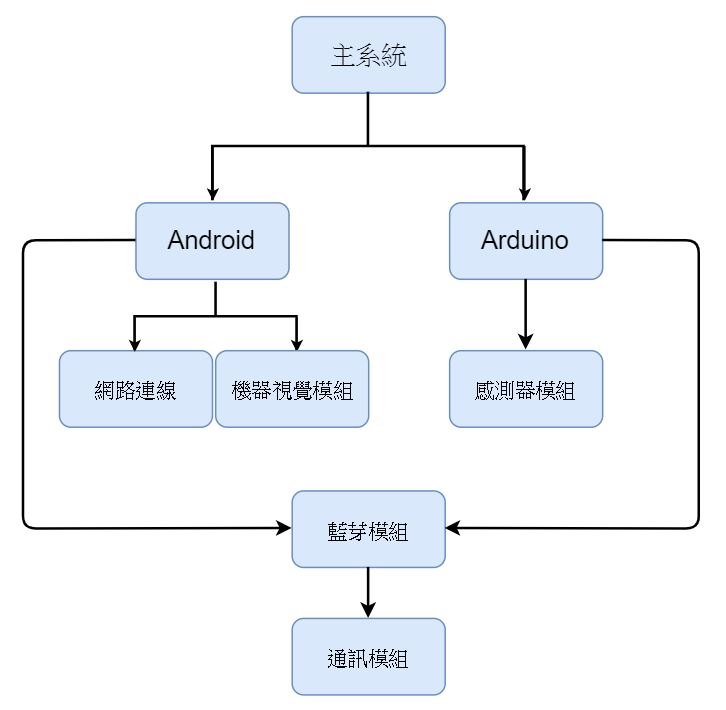
\includegraphics[width=10cm]{pic/ch2/軟硬體架構圖.JPG}
\caption{軟硬體架構圖} \label{軟硬體架構圖}
\end{figure}

\subsection{硬體架構}

\subsubsection{系統外觀介紹}
本系統外觀分別為Android手持裝置、肌肉感測器、藍芽裝置、電源四項,介紹如下:
\begin{enumerate}
\item Android手持裝置(圖 \ref{Android}):本專題使用到手機上的相機、藍芽功能。
\item 肌肉感測器(圖 \ref{MuscleSensor}):
\begin{itemize}
\item 供電電壓:+3.1V\textasciitilde +5V
\item RAW EMG 輸出:MyoWare 能擁有二次輸出 RAW EMG 波形的機會。
\item LED 指示燈:增加兩個版載LED燈,當MyoWare的電源鍵是開的,肌肉用力時LED燈即會發亮。
\end{itemize}
\item 藍芽裝置(圖 \ref{Bluetooth}):藍芽模組可以與手持裝置的藍芽互相傳送接收訊息。
\item 電源(圖 \ref{MobilePower}):使用電流穩定既可重複使用的行動電源作為供電來源。
\end{enumerate}

\begin{figure}[h]  % Put pictures here.
\subfigure[Android手持裝置]{
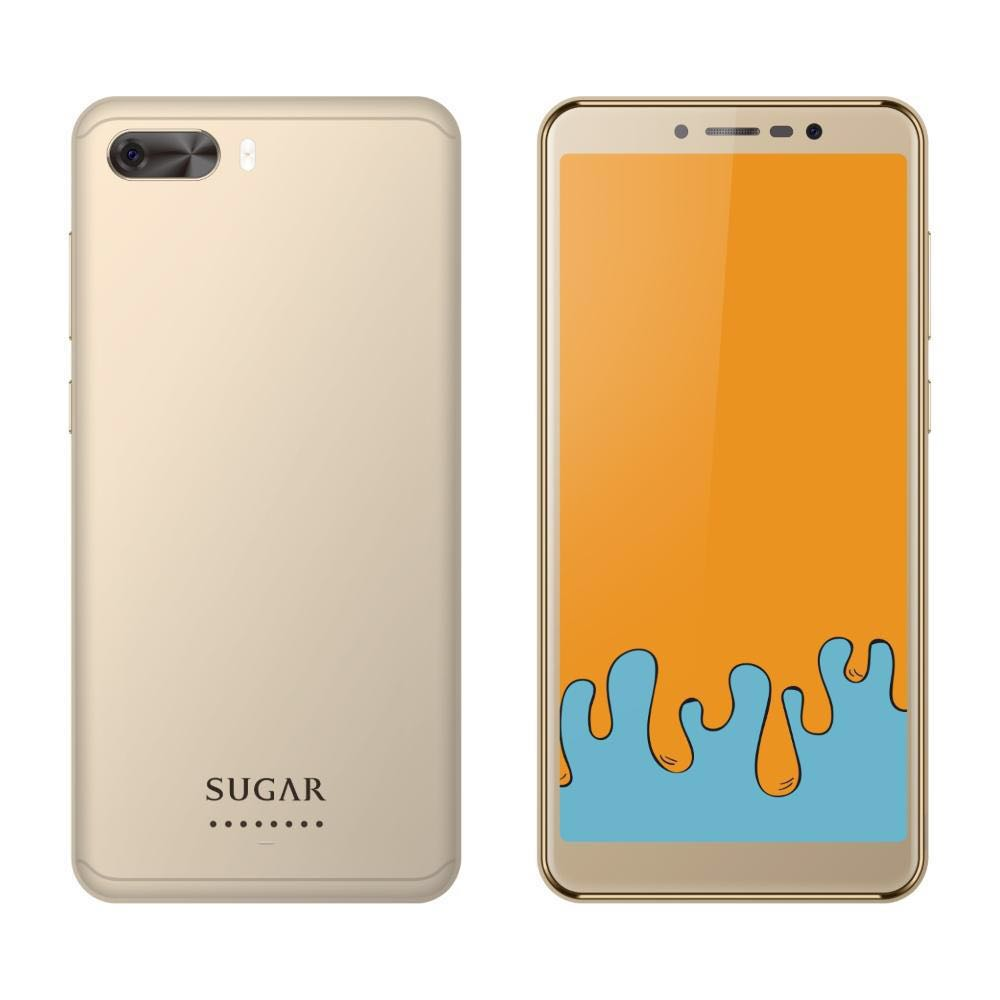
\includegraphics[width=3cm]{pic/ch2/Android.jpg}
\label{Android}
}
\quad
\subfigure[肌肉感測器]{
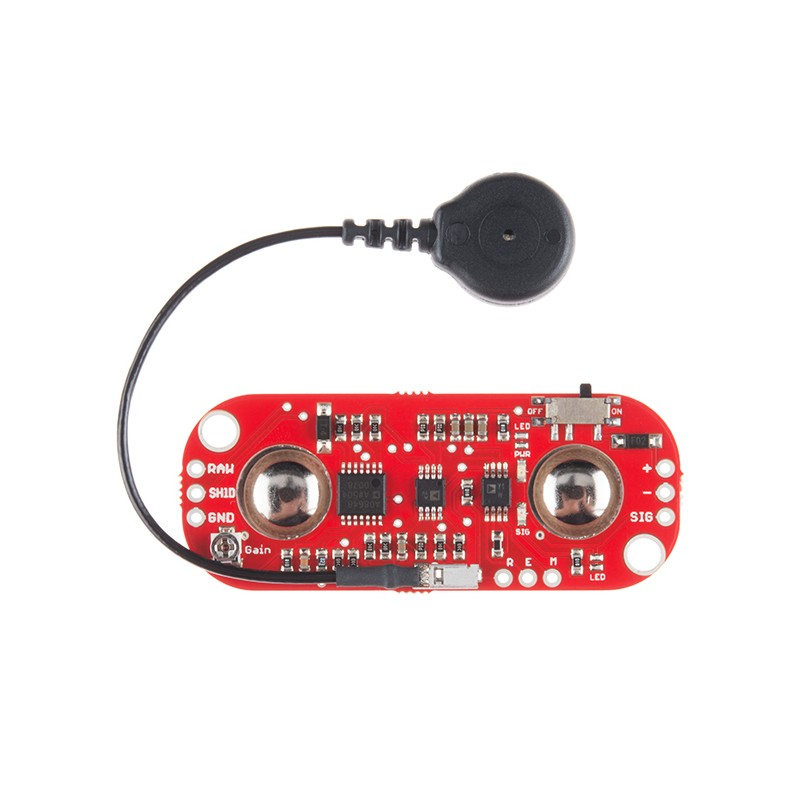
\includegraphics[width=3cm]{pic/ch2/MuscleSensor.jpg}
\label{MuscleSensor}
}
\quad
\subfigure[藍芽裝置]{
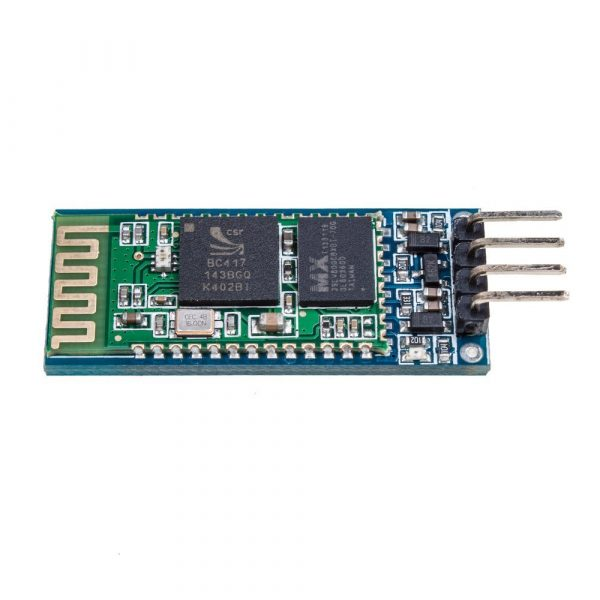
\includegraphics[width=3cm]{pic/ch2/Bluetooth.jpg}
\label{Bluetooth}
}
\quad
\subfigure[電源]{
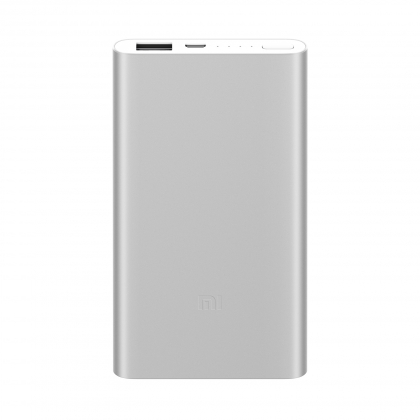
\includegraphics[width=3cm]{pic/ch2/MobilePower.jpg}
\label{MobilePower}
}
\caption{系統外觀介紹}
\end{figure}

\begin{figure}[h]  % Put pictures here.
\centering
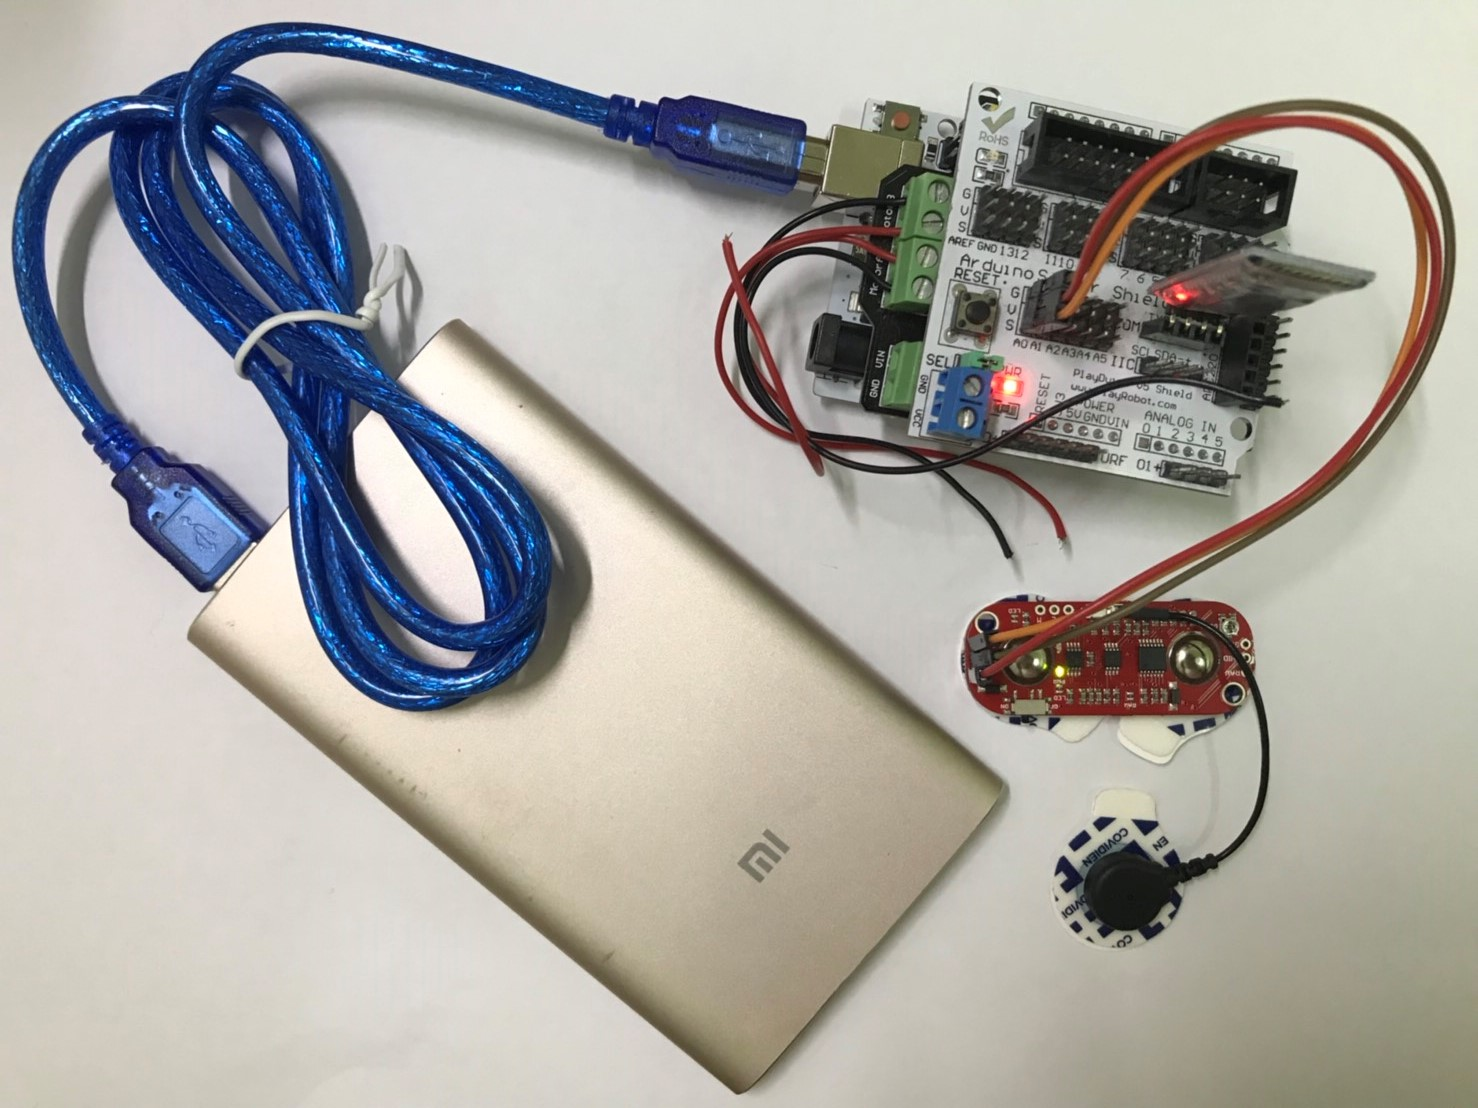
\includegraphics[width=5cm]{pic/ch2/HardwareSystem.jpg}
\caption{硬體系統整合}
\end{figure}

\subsubsection{感測技術}
製作本系統所需主要技術如下:
\begin{enumerate}
\item 肌肉感測器
\begin{itemize}
\item 通過 MyoWare 可以測量肌肉的電訊號活動,在過去實驗一般稱之為肌電儀器(EMG)。當大腦下指令告訴你的肌肉收縮,將發送一個傳遞路徑提醒肌肉開始徵招肌肉運動單元(肌束纖維使肌肉產生力量)。當肌肉越用力,產生越多的肌肉運動單元來招募更大的肌肉力量。當招募越多的肌肉單元數目,將會產生更多的肌肉電位改變。MyoWare 將分析此電訊號並輸出訊號來表示肌肉如何用力。當你越用力 MyoWare 將輸出更大的電壓。雖然 EMG 已能偵測肌肉放電的訊號,但 MyoWare 則使它更具意義更為人性化。
\item 我們以 0.15 秒讀取一次的頻率取得訊號,以 1.2 秒為一個間距分析其中的變化。之後在第三章會對感測器訊號分析的演算法有更詳細地介紹。
\item 圖 \ref{感測器流程圖} 為感測器流程圖
\begin{figure}[h]  % Put pictures here.
\centering
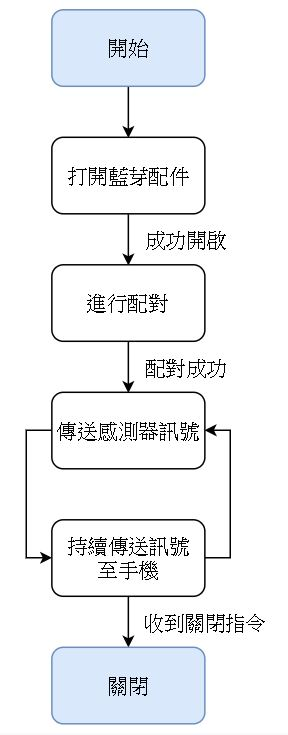
\includegraphics[width=4cm]{pic/ch2/感測器流程圖.JPG}
\caption{感測器流程圖} \label{感測器流程圖}
\end{figure}
\end{itemize}

\item Android 藍芽連接
\begin{itemize}
\item 使用無線通訊的概念,藉由藍芽通訊,手持裝置得以與肌肉感測器相互傳遞訊息。
\item 藍芽開啟之操作流程:
\begin{description}
\item [Step1.] 打開手持裝置藍芽。
\item [Step2.] 點選「HC-06」進行配對。
\item [Step3.] 回到應用程式主畫面,點選藍芽連線。
\item [Step4.] 顯示連線成功。
\end{description}
\item 圖 \ref{藍芽開啟流程圖} 為藍芽開啟流程圖
\begin{figure}[h]  % Put pictures here.
\centering
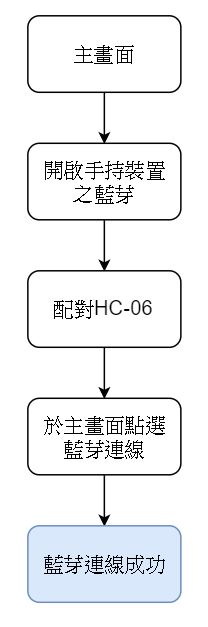
\includegraphics[width=3cm]{pic/ch2/藍芽開啟流程圖.JPG}
\caption{藍芽開啟流程圖} \label{藍芽開啟流程圖}
\end{figure}
\end{itemize}

\item Android 相機
\begin{itemize}
\item 我們使用 OpenCV Android SDK 提供的 JavaCameraView 來調用 android 相機。JavaCameraView 繼承 Android 內建SurfaceView 但必須呼叫 onCameraFrame 來取得每帧相機影像來供後續 OpenCV 程式庫處裡。OpenCV(Open Source Computer Vision Library) 是一套跨平台的電腦視覺式庫,支援圖像處裡、電腦視覺和模式識別的程式開發。在本專題中我們使用 OpenCV的臉部偵測及影像縫合功能將圖示縫合於臉部畫面上,以達到擴增實境的效果。
\end{itemize}
\end{enumerate}

\subsection{軟體架構}
軟體部分中包含了網路連線功能、藍芽功能、Arduino端功能以及遊戲端功能,接下來會依序介紹其用途及操作流程。

\subsubsection{網路連線功能}
\begin{itemize}
\item 基於TCP網路架構,建構出Server端及Player(Client)端,使影像與數據以此通道傳輸。
\item 使用不同 Thread 分別執行 inputstream 與outputstream,於網路通道上進行輸入及輸出,且以 lock、unlock、await、signal 處理同步問題。
\item 圖 \ref{網路協定圖} 為網路協定圖
\begin{figure}[htbp]
\subfigure[Player連線協定圖]{
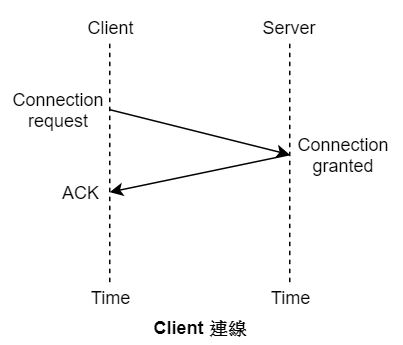
\includegraphics[width=7cm]{pic/ch2/tcp01.JPG}
}
\quad
\subfigure[Player結束連線協定圖]{
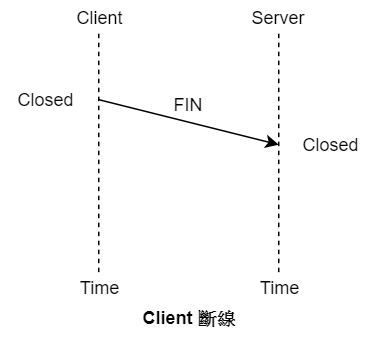
\includegraphics[width=7cm]{pic/ch2/tcp02.JPG}
}
\quad
\subfigure[Player傳送、接收影像協定圖]{
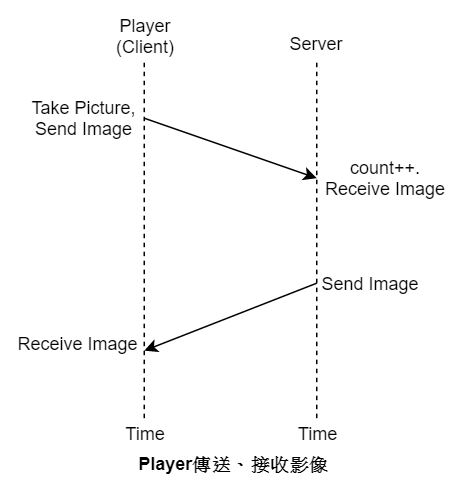
\includegraphics[width=7cm]{pic/ch2/tcp03.JPG}
}
\caption{網路協定圖} \label{網路協定圖}
\end{figure}
\newpage

\item 以下為Server端之程式碼片段
\begin{itemize}
\item 圖 \ref{S建立連線} 為建立連線
\begin{figure}[htbp]
\centering
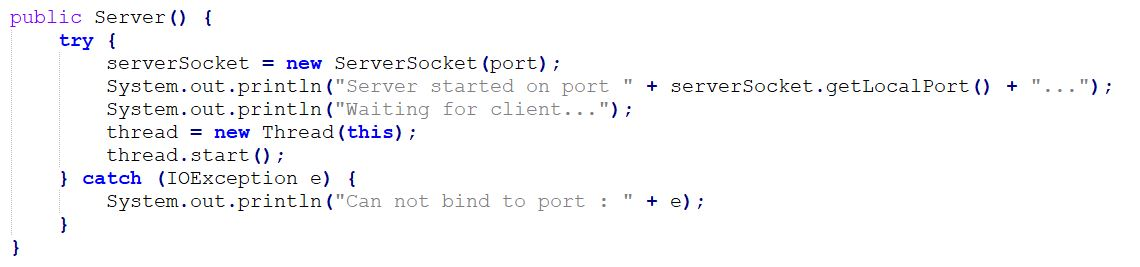
\includegraphics[width=10cm]{pic/ch2/code-Server.JPG}
\caption{建立連線} \label{S建立連線}
\end{figure}
\item 圖 \ref{S接收數據} 為接收數據
\begin{figure}[htbp]
\centering
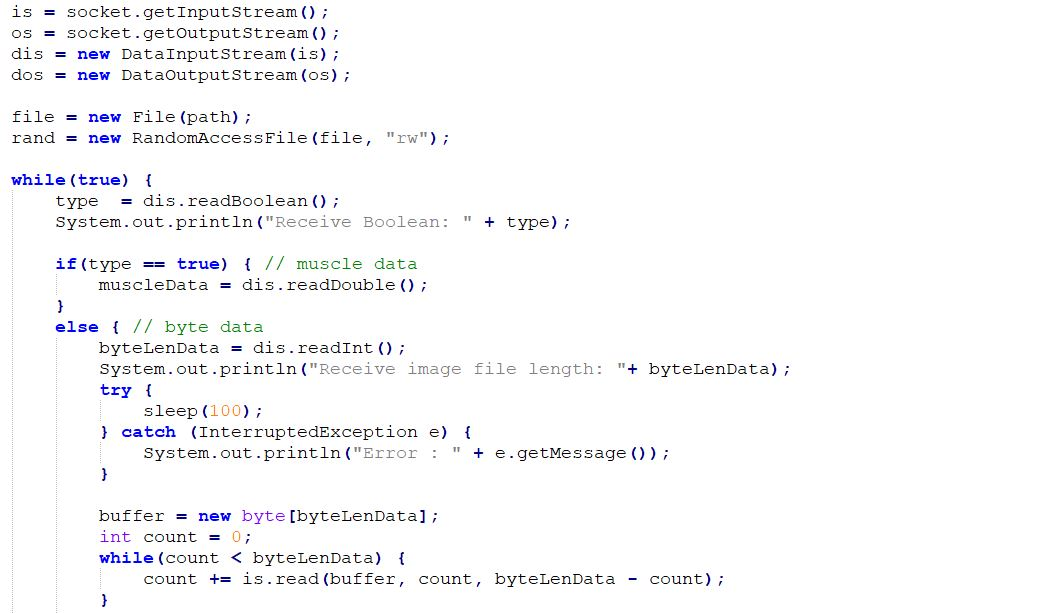
\includegraphics[width=10cm]{pic/ch2/code-Server2.JPG}
\caption{接收數據} \label{S接收數據}
\end{figure}
\item 圖 \ref{S傳送數據} 為傳送數據
\begin{figure}[htbp]
\centering
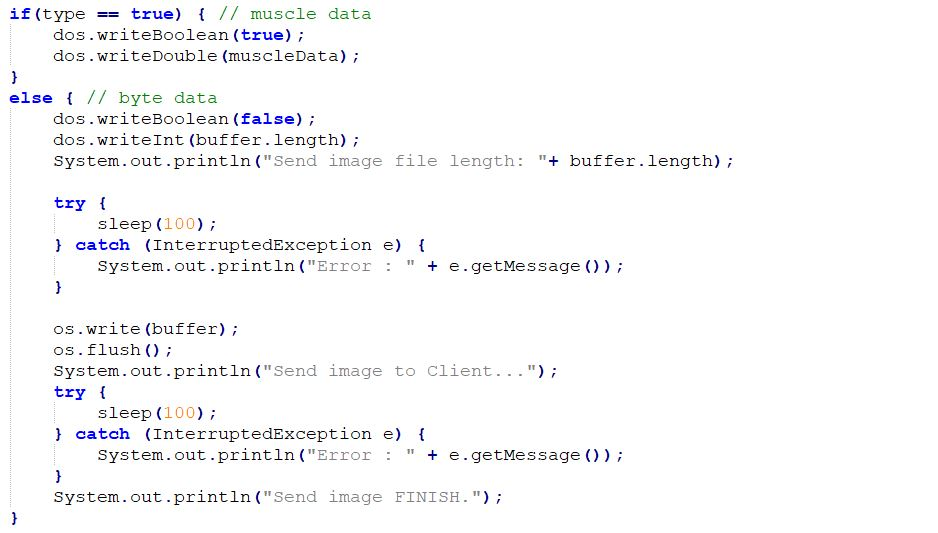
\includegraphics[width=10cm]{pic/ch2/code-Server3.JPG}
\caption{傳送數據} \label{S傳送數據}
\end{figure}
\end{itemize}
\newpage

\item 以下為Client端之程式碼片段
\begin{itemize}
\item 圖 \ref{C建立連線} 為建立連線
\begin{figure}[htbp]
\centering
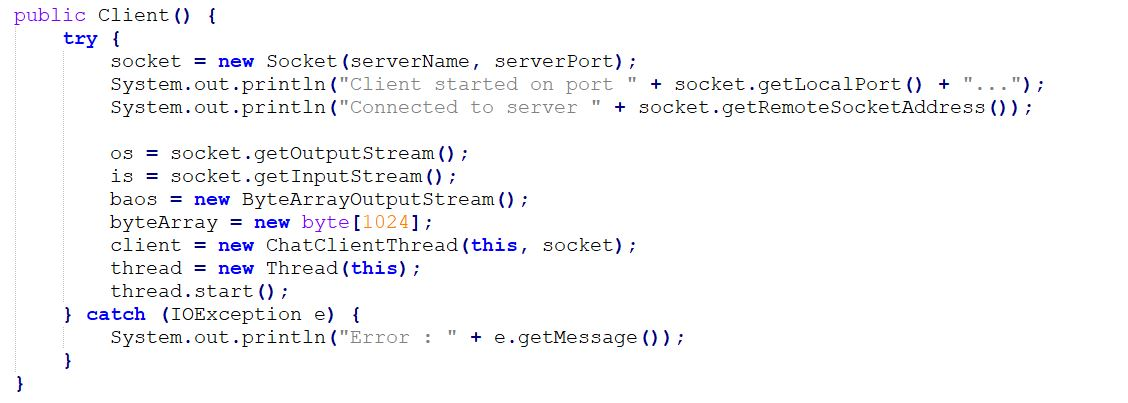
\includegraphics[width=10cm]{pic/ch2/code-Client.JPG}
\caption{建立連線} \label{C建立連線}
\end{figure}
\item 圖 \ref{C傳送數據} 為傳送數據
\begin{figure}[htbp]
\centering
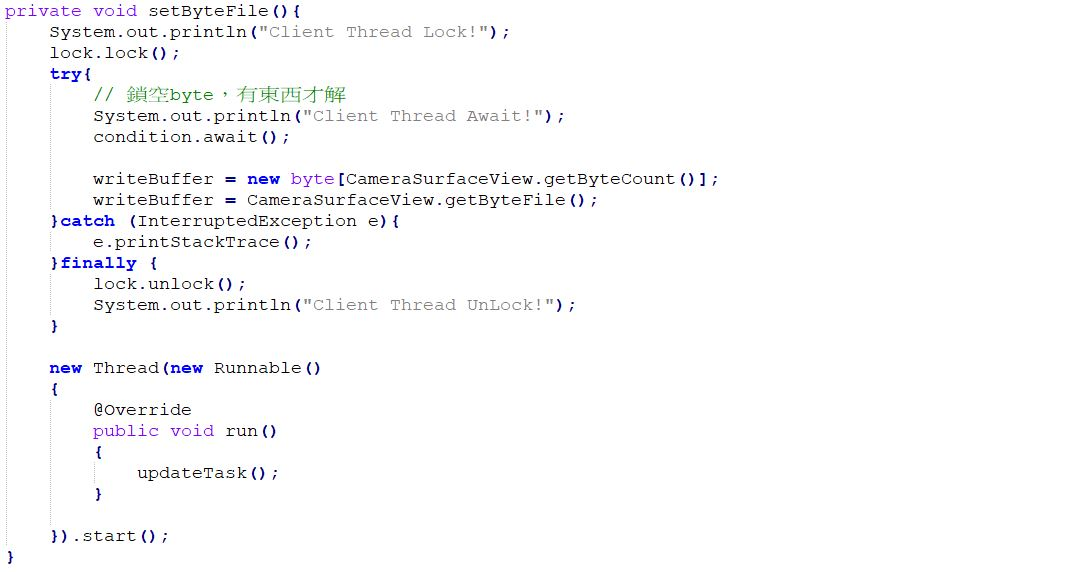
\includegraphics[width=10cm]{pic/ch2/code-Client2.JPG} \\ 
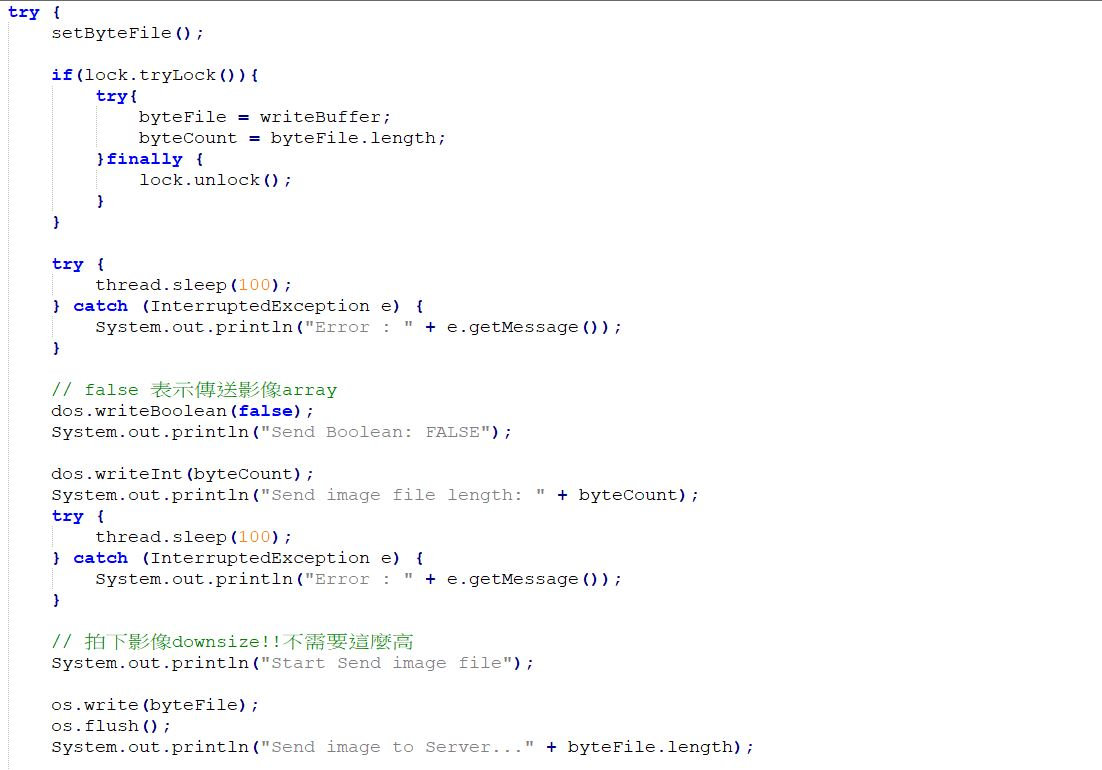
\includegraphics[width=10cm]{pic/ch2/code-Client3.JPG}
\caption{傳送數據} \label{C傳送數據}
\end{figure}
\item 圖 \ref{C接收數據} 為接收數據
\begin{figure}[htbp]
\centering
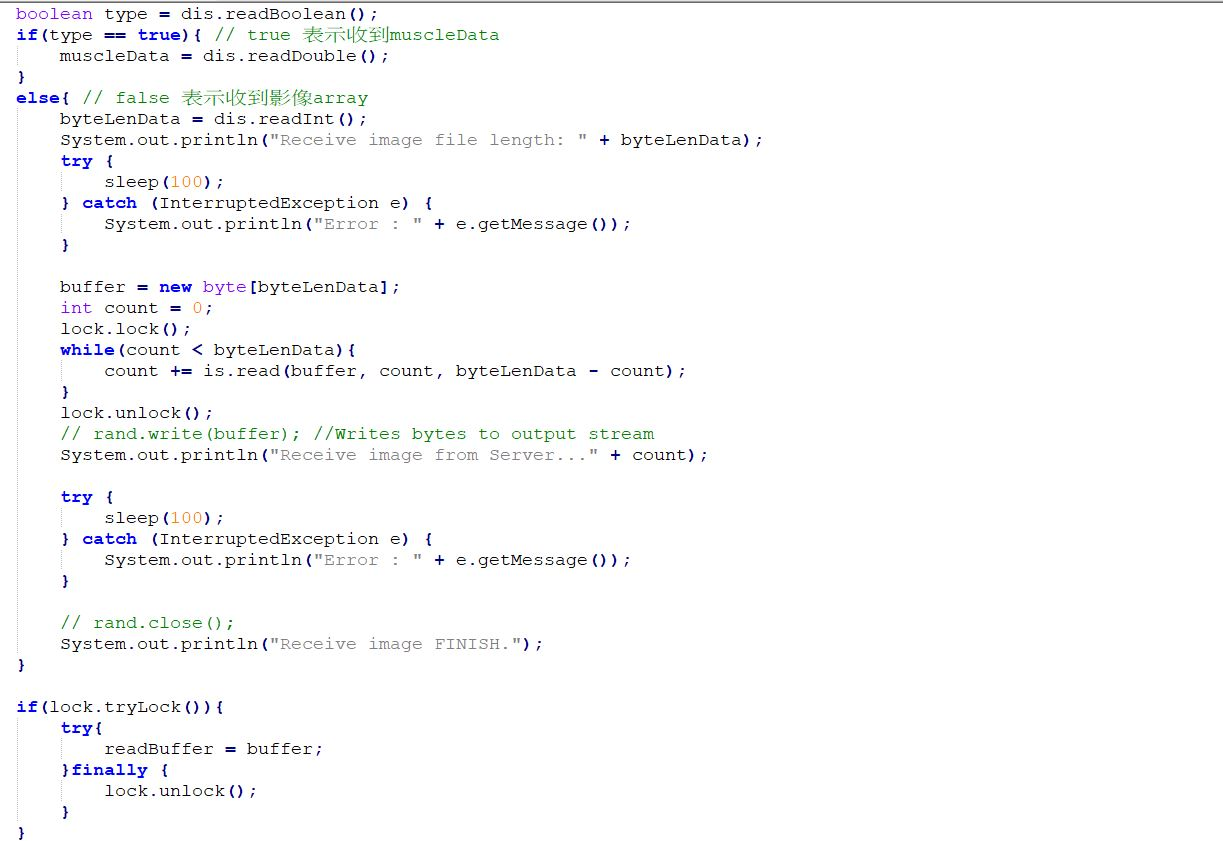
\includegraphics[width=10cm]{pic/ch2/code-Client4.JPG}
\caption{接收數據} \label{C接收數據}
\end{figure}
\end{itemize}
\newpage
\end{itemize}

\subsubsection{藍芽功能}
\begin{itemize}
\item 用途為建立與肌肉感測器之間的通訊。
\item 圖 \ref{藍芽連線之程式碼片段} 為將藍芽連線至裝置之程式碼片段。
\begin{figure}[htbp]
\centering
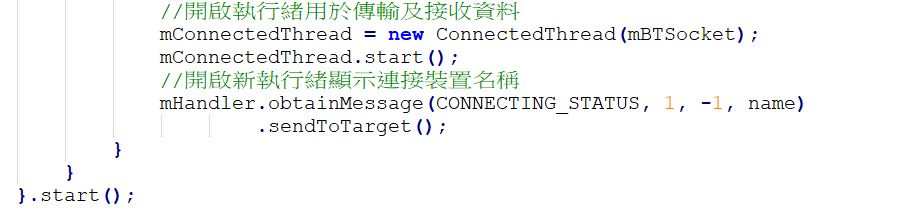
\includegraphics[width=15cm]{pic/ch2/code-BluetoothActivity.JPG}
\caption{藍芽連線之程式碼片段} \label{藍芽連線之程式碼片段}
\end{figure}

\item 圖 \ref{藍芽接收之程式碼片段} 為藍芽接收訊號,以 byte 形式儲存,並且將收到的數字存在session 以便之後的計算。
\begin{figure}[htbp]
\centering
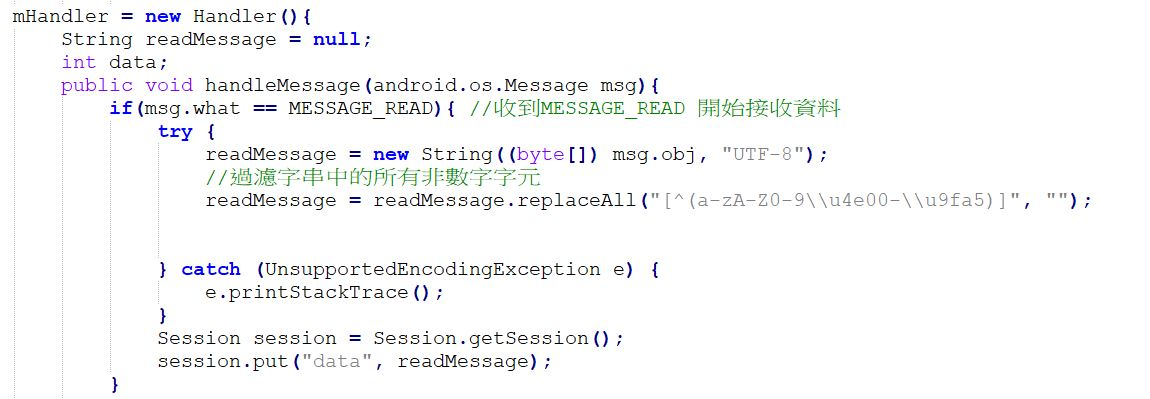
\includegraphics[width=15cm]{pic/ch2/code-BluetoothActivity2.JPG}
\caption{藍芽接收之程式碼片段} \label{藍芽接收之程式碼片段}
\end{figure}
\end{itemize}

\subsubsection{Arduino端功能}
\begin{itemize}
\item 將肌肉感測器輸出線路插在指定腳位,之後將貼片貼在手臂的指定位置上。
\item 圖 \ref{Arduino之程式碼片段} 為將感測器訊號由 Arduino 端傳至 Android 手機端之程式碼片段。
\begin{figure}[htbp]
\centering
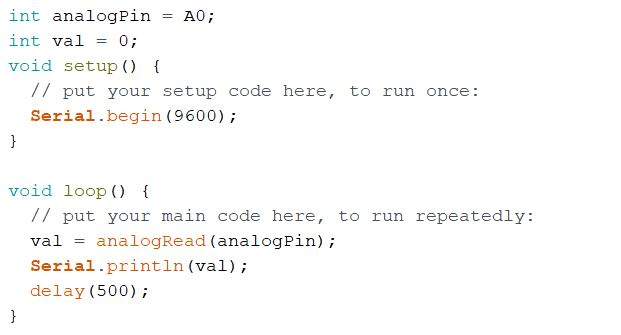
\includegraphics[width=10cm]{pic/ch2/code-Arduino.JPG}
\caption{Arduino之程式碼片段} \label{Arduino之程式碼片段}
\end{figure}
%\item 圖為在手機端能清楚讀入感測器傳入的數值。
\end{itemize}
\newpage

\section{肌肉感測訊號分析與影像處理}
本章節著重介紹肌肉感測訊號分析與影像處理技術。描述這些功能包含目的、演算法流程與程式碼片段說明。

\subsection{肌肉感測器訊號分析}
\begin{itemize}
\item 目的:用於分析由 Arduino 傳至手持裝置的肌肉感測器訊號。過濾不可用的訊號後,利用快速傅立葉轉換得知訊號的大小與頻率。
\item 演算法流程
\begin{itemize}
\item 如圖 \ref{陣列與訊號關係示意圖} 所示,陣列一為隨時更新最新資訊的短陣列(紅色),陣列二為隨時更新最新訊號的長陣列(綠色)。下面會說明兩個陣列分別執行的不同計算工作。
\begin{figure}[htbp]
\centering
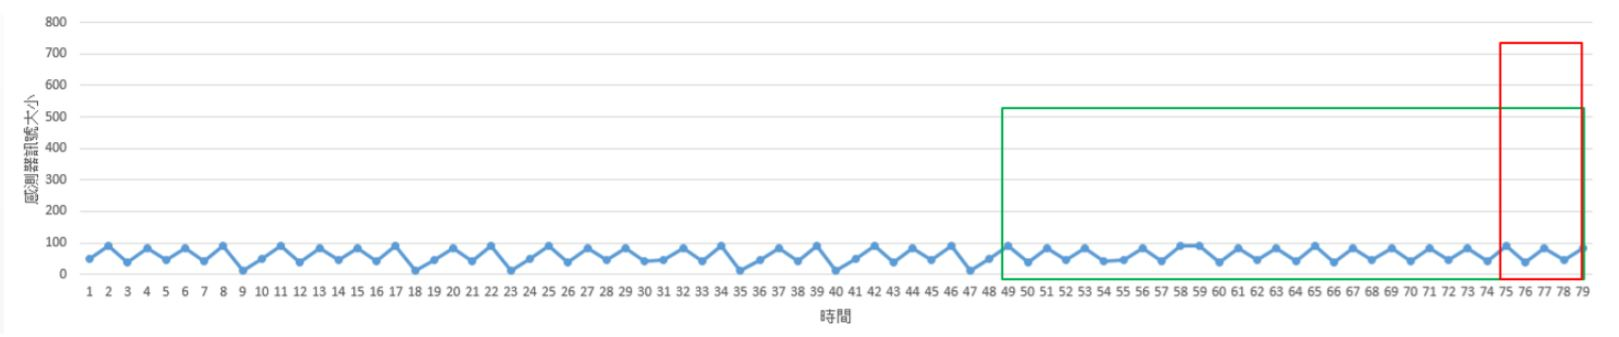
\includegraphics[width=15cm]{pic/ch3/陣列與訊號關係示意圖.JPG}
\caption{陣列與訊號關係示意圖} \label{陣列與訊號關係示意圖}
\end{figure}

\item 如圖 \ref{部分程式碼片段} 所示,在大的陣列裝滿後,以小的陣列用於判斷訊號是否在變化,有的話就以大的陣列判斷變換的節奏。
\begin{figure}[htbp]
\subfigure[設兩個分別為大跟小的陣列]{
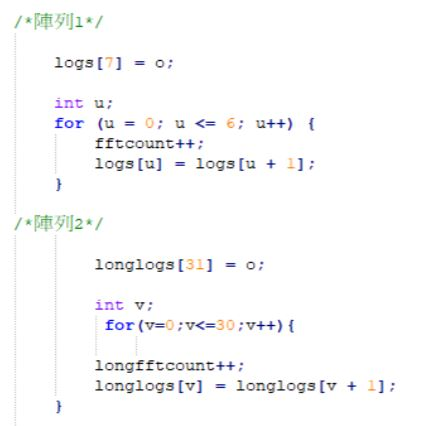
\includegraphics[width=7cm]{pic/ch3/設兩個分別為大跟小的陣列.JPG}
}
\quad
\subfigure[開始執行]{
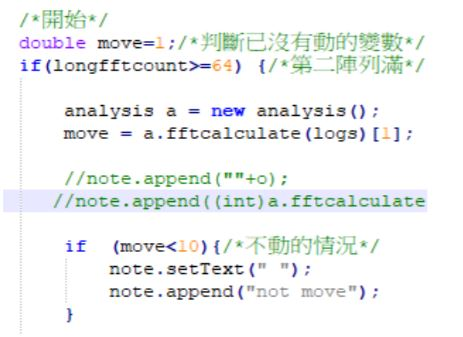
\includegraphics[width=7cm]{pic/ch3/開始執行.JPG}
}
\caption{部分程式碼片段} \label{部分程式碼片段}
\end{figure}

\item 如圖 \ref{訊號頻率} 所示,轉換後的結果較轉換前容易判斷頻率,在遊戲的演算法中可以較容易的定義肌肉放鬆節奏的快慢。
\begin{figure}[htbp]
\subfigure[轉換前之訊號]{
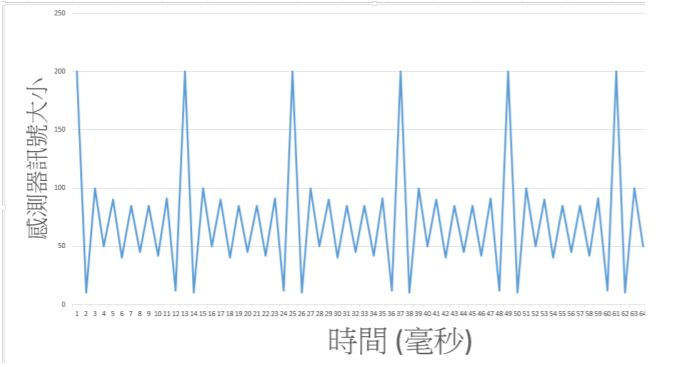
\includegraphics[width=7cm]{pic/ch3/轉換前之訊號.JPG}
}
\quad
\subfigure[轉換後之訊號]{
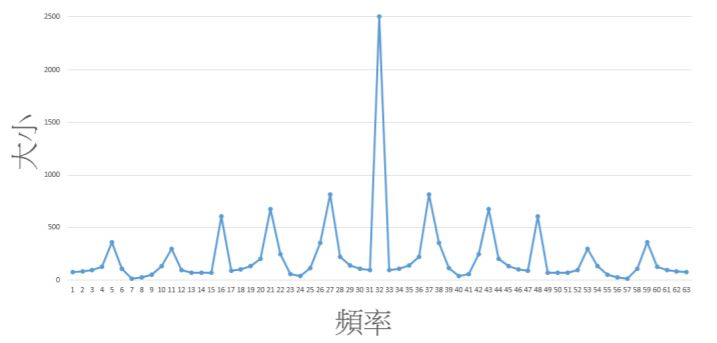
\includegraphics[width=7cm]{pic/ch3/轉換後之訊號.JPG}
}
\caption{訊號頻率} \label{訊號頻率}
\end{figure}

\item 如圖 \ref{快速傅立葉之程式碼片段} 所示,傅立葉轉換主要的功能是用於信號在時域(或空域)和頻域之間的變換。我們用轉換後的結果來判斷訊使用者行為有沒有在動,然後再用另一個更長的來判斷使用者行為,這樣做的目的是減少延遲的時間。
\begin{figure}[htbp]
\centering
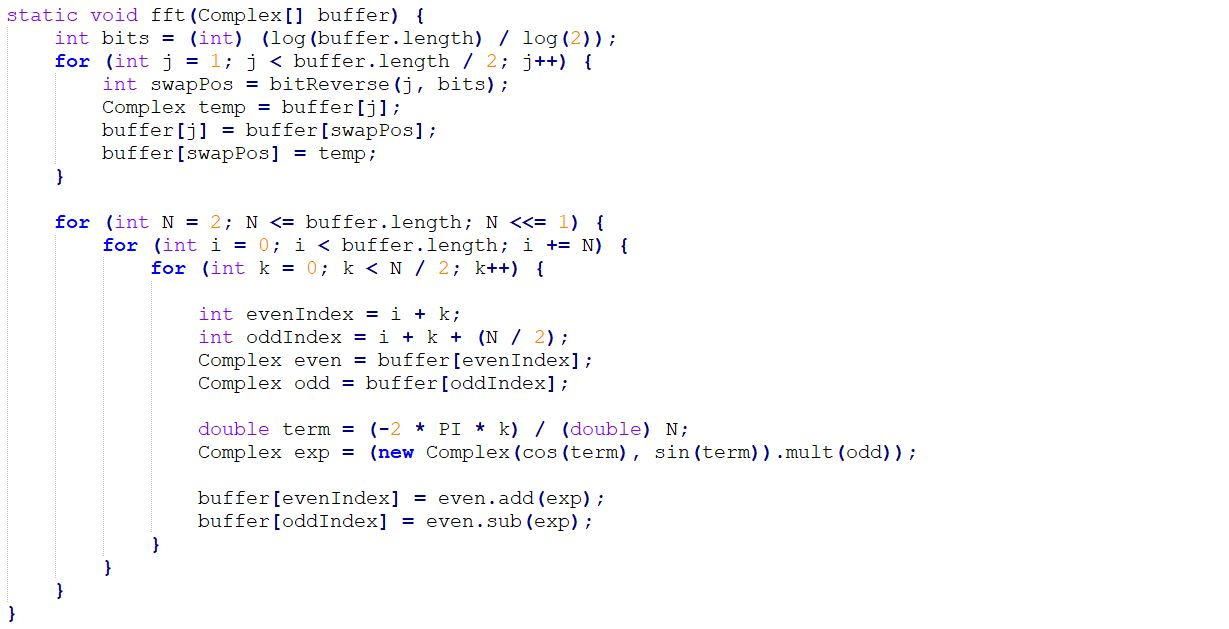
\includegraphics[width=15cm]{pic/ch3/code-快速傅立葉.JPG}
\caption{快速傅立葉之程式碼片段} \label{快速傅立葉之程式碼片段}
\end{figure}
\newpage

\item 如圖 \ref{速度分級之程式碼片段} 所示,將速度分為三個階段,越快的會加分的越快。
\begin{figure}[htbp]
\centering
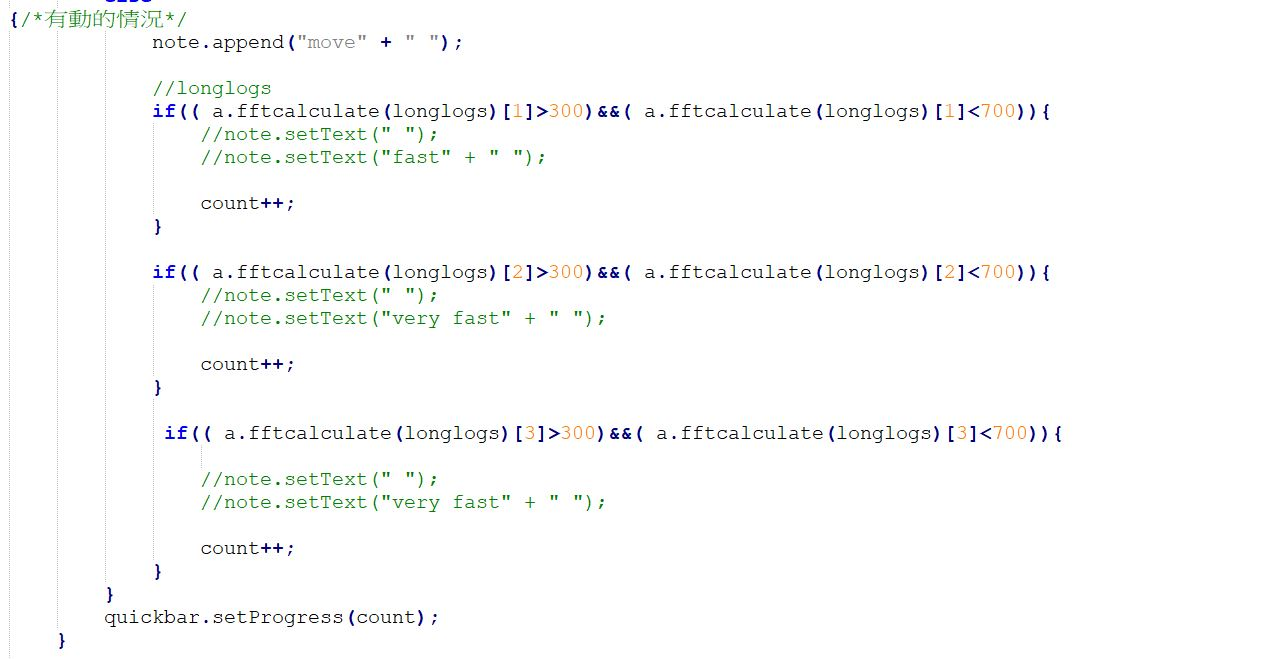
\includegraphics[width=15cm]{pic/ch3/code-速度分級.JPG}
\caption{速度分級之程式碼片段} \label{速度分級之程式碼片段}
\end{figure}
\end{itemize}
\end{itemize}
\newpage

\subsection{影像處理}
\subsubsection{使用工具}
\begin{itemize}
\item 使用Google Firebase ML Kit。ML Kit為Google 在2018年新開發出專為行動裝置所設計的SDK。主要將Google Cloud Vision API、Mobile Vision、Tensorflow Lite三部分組合而成。本次專題中主要使用到ML Kit 提供的影像相關之Vision API 的Face Detection部分。
\item Face Detection API之特點
\begin{description}
\item[1] 能快速辨識並且標記出臉部的特徵點:能辨識出各臉部中五官之位置及人臉或五官之輪廓。
\item[2] 辨識臉部表情:能辨識臉部是否在微笑、是否閉上眼睛。
\item[3] 人臉追蹤:辨識影片曾出現過的人臉,並給予ID以便讀取關於某面孔之資料。
\item[4] 即時處理:即使在沒有網路服務下仍能快速處理辨識。在動態畫面的處理上效能更佳。
\end{description}
\end{itemize}

\subsubsection{特徵點提取及臉部偵測技術}
\begin{itemize}
\item 臉部偵測概述
\begin{description}
\item[1] Face Orientation
\begin{itemize}
\item 臉部偵測的第一步為偵測臉部之位置,並找出其轉向的角度。(圖 \ref{Pose angle estimation} 所示)
\begin{figure}[htbp]
\subfigure[The coordinate system]{

\includegraphics[width=5cm]{pic/ch3/coord.png}
}
\quad
\subfigure[Pose angle examples]{
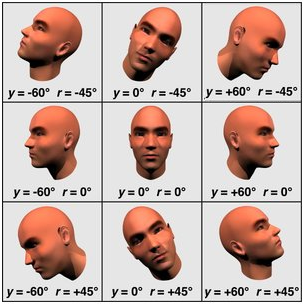
\includegraphics[width=5cm]{pic/ch3/poseangles.png}
}
\caption{Pose angle estimation} \label{Pose angle estimation}
\end{figure}
\item API中所檢測到的為Euler Y 以及 Euler Z。預設回傳Euler Z,如果需取得Euler Y則需將檢測器之設定做修改。
\end{itemize}

\item[2] Landmarks
\begin{itemize}
\item 此為面部中的特徵點,例如左右眼、鼻頭皆為此。
\item 在此API中,偵測時並沒有先以特徵點來做為面部偵測的基礎,而是先將臉部整體偵測出來後從中提取出所需要的Landmarks。
\item 其中因不同的Euler Z所能偵測的也會有所不同。詳細如下圖 \ref{Landmark與EulerZ之關係圖} 所示。
\begin{figure}[htbp]
\centering
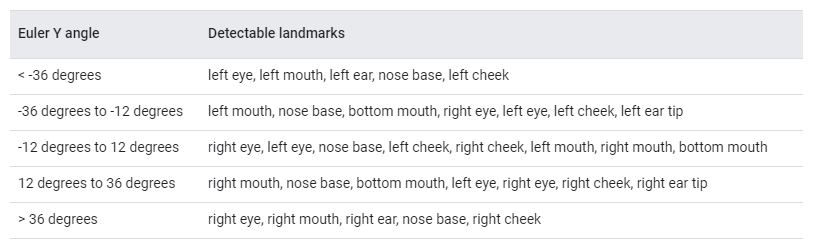
\includegraphics[width=10cm]{pic/ch3/Landmarks.JPG}
\caption{Landmark與Euler Z之關係圖} \label{Landmark與EulerZ之關係圖}
\end{figure}
\end{itemize}

\item[3] Contours \\
將代表面部特徵之點組合而形成的輪廓,而所偵測到的特徵輪廓都由特定數量的點來表示,而當面部中總共133個Contours 皆取得時,每個特徵輪廓皆會有特定的編號。(圖 \ref{特徵點相關資訊} 及圖 \ref{所偵測之結果} 所示 )
\begin{figure}[htbp]
\subfigure[特徵輪廓數量]{
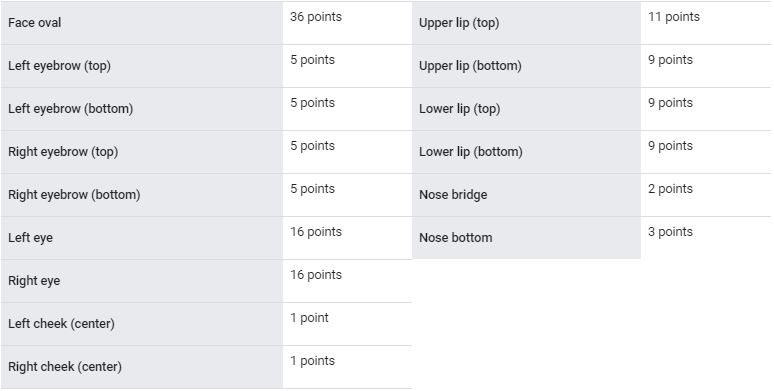
\includegraphics[width=5cm]{pic/ch3/numberOfPoints.JPG}
}
\quad
\subfigure[Landmark的編號]{
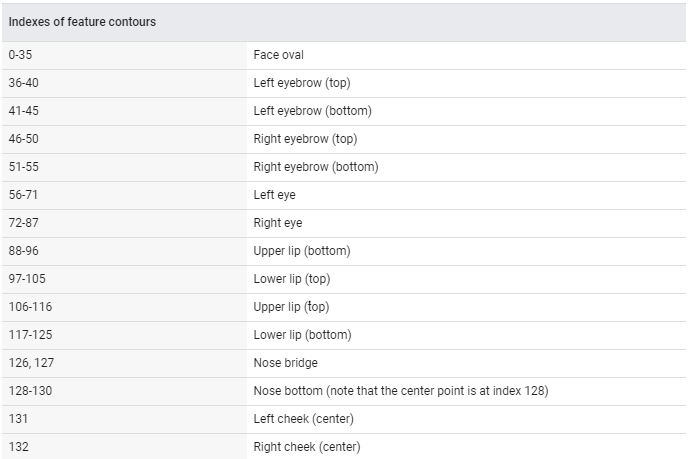
\includegraphics[width=5cm]{pic/ch3/feature_contours.JPG}
}
\caption{特徵點相關資訊} \label{特徵點相關資訊}
\end{figure}
\begin{figure}[htbp]
\centering
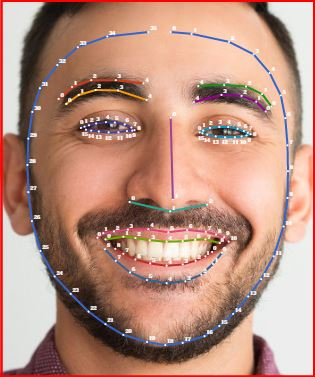
\includegraphics[width=5cm]{pic/ch3/face_contours.JPG}
\caption{所偵測之結果} \label{所偵測之結果}
\end{figure}
\end{description}
\end{itemize}
\newpage

\subsubsection{ML Kit 運行步驟}
\begin{itemize}
\item 前置步驟及基本需求
\begin{description}
\item[1] 將所需之firebase檔案新增近專案中
\item[2] 為了使面部偵測更加準確,在圖像中至少需要100x100像素以偵測到臉部區域,如要更精確地獲得輪廓資訊則需要200x200像素。
\end{description}

\item 運行步驟
\begin{description}
\item[1] 建立檢測器FirebaseVisionFaceDetectorOptions
\begin{itemize}
\item 在將人臉檢測應用於圖像之前,可更改人臉檢測器的默認設置。例如是否識別Landmarks亦或是在模式中對於速度及準確度兩者的優先。
\item 以圖 \ref{DetectorOptions} 解釋,在此檢測器中因為即時影像傳送,故以速度作為優先選擇。
\begin{figure}[htbp]
\centering
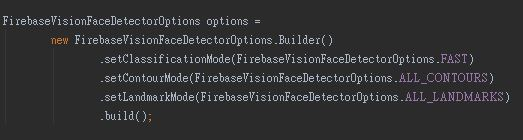
\includegraphics[width=10cm]{pic/ch3/DetectorOptions.JPG}
\caption{程式碼截圖} \label{DetectorOptions}
\end{figure}
\end{itemize}

\item[2] 將資料轉成檢測器所需之圖像物件FirebaseVisionImage
\begin{itemize}
\item FirebaseVisionImage extends Object
\item 能將不同的資料型態轉變為可用於偵測器的物件,但不同的資料性態在轉換時會擁有不同的需求,例如ByteBuffery在轉換時需要先將物件轉換成FirebaseVisionImageMetadata物件來進行描述。(圖 \ref{VisionImage})
\begin{figure}[htbp]
\centering
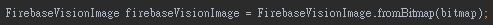
\includegraphics[width=10cm]{pic/ch3/VisionImage.JPG}
\caption{程式碼截圖} \label{VisionImage}
\end{figure}
\end{itemize}

\item[3] 執行檢測器FirebaseVisionFaceDetector(圖 \ref{detector})
\begin{figure}[htbp]
\centering
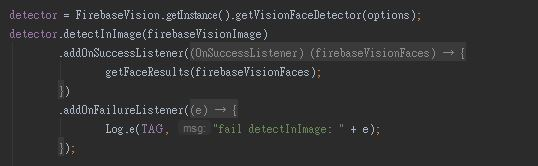
\includegraphics[width=10cm]{pic/ch3/detector.JPG}
\caption{程式碼截圖} \label{detector}
\end{figure}

\item[4] 取得偵測完之物件FirebaseVisionFace(圖 \ref{FaceResult})
\begin{figure}[htbp]
\centering
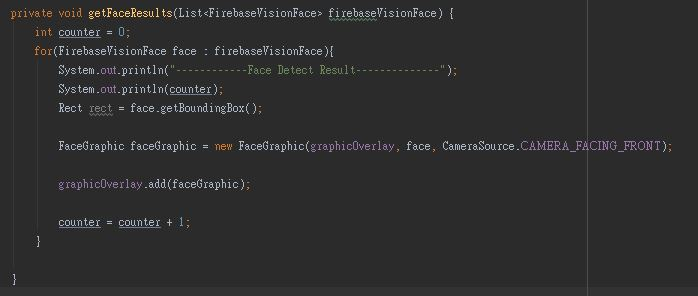
\includegraphics[width=10cm]{pic/ch3/FaceResult.JPG}
\caption{程式碼截圖} \label{FaceResult}
\end{figure}
在FirebaseVisionFace便存取了在臉部改動所需要的臉部輪廓座標以及面部特徵輪廓座標資料。
\end{description}
\end{itemize}

\subsubsection{面部更改}
\newpage


\section{實驗結果}
本章節將實際展示此專題成果,並依序分析各項功能在實驗環境下的結果,包含:網路傳送延遲時間之計算評估、影像處理精確度及延遲之評估、肌肉感測器延遲評估。此外,講述實作的過程,以及在實作途中所遭遇到的問題與解決方式,並附上遊戲者體驗之評價。

\subsection{實驗環境}
本系統的硬體設備與軟體開發環境
\begin{itemize}
\item 手持裝置:Android 8.0.0, RAM:4GB
\item 相機視覺處理技術:OpenCV 3.1.0
\item Arduino 程式開發環境:Ardunio 1.6.12
\item Android 程式開發環境:Android Studio 2.3
\end{itemize}

\subsection{網路傳送延遲時間之計算評估}
網路傳送延遲時間之計算評估

\subsection{影像處理精確度及延遲之評估}
影像處理精確度及延遲之評估

\subsection{肌肉感測器延遲評估}
肌肉感測器延遲評估

\subsection{專題結果展示}
\begin{itemize}
\item 遊戲主頁面及開始畫面(連線上Server) \\ \\
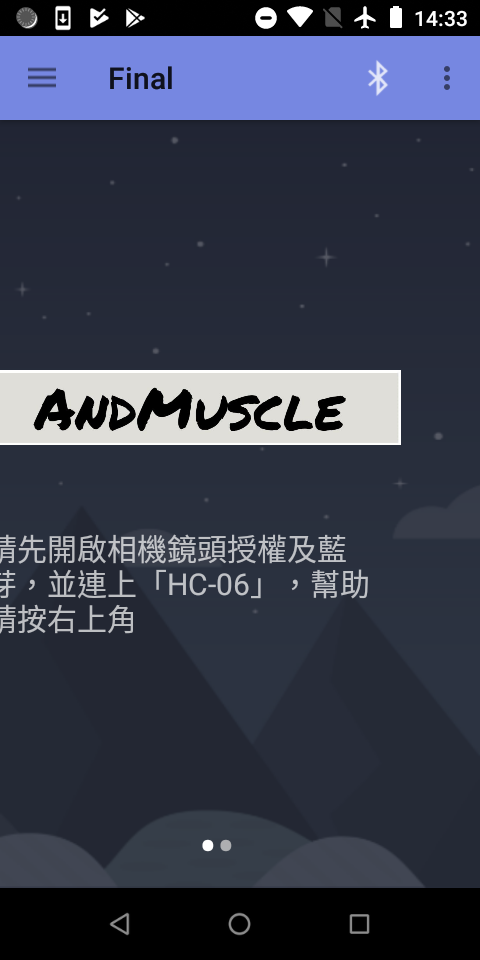
\includegraphics[scale=0.15]{pic/ch4/game01.png} 
\space \space
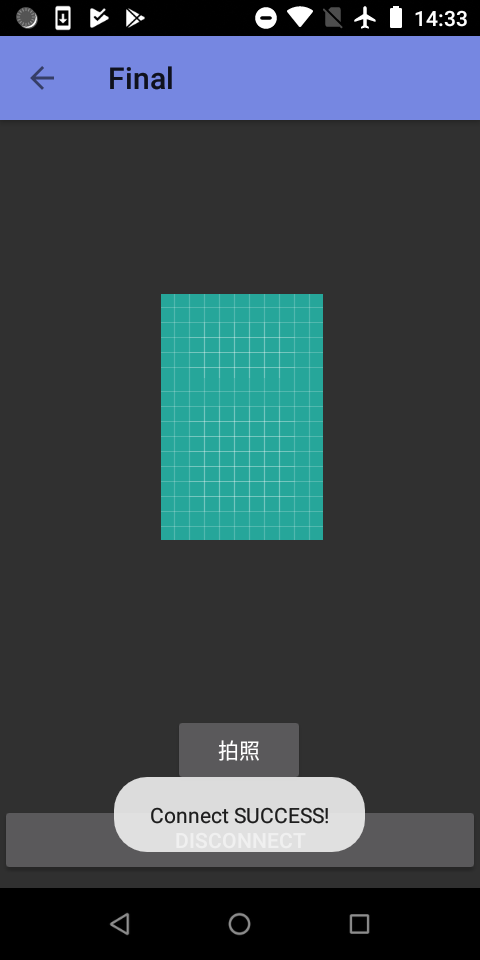
\includegraphics[scale=0.15]{pic/ch4/game02.png}
\item 遊戲中畫面 \\ \\
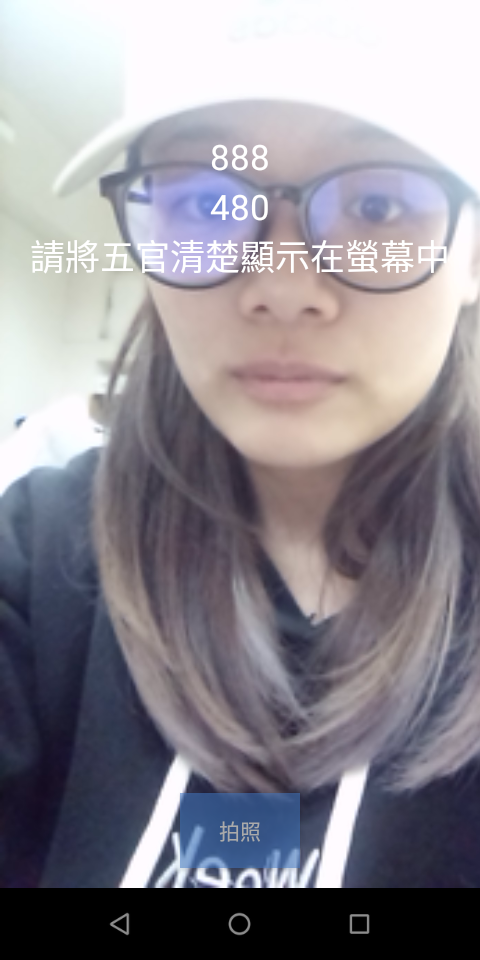
\includegraphics[scale=0.15]{pic/ch4/game03.png}
\space \space
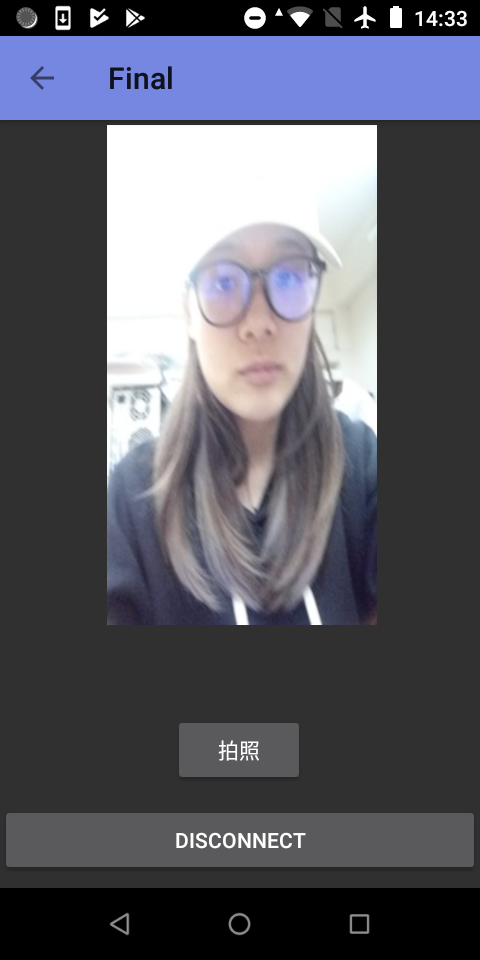
\includegraphics[scale=0.15]{pic/ch4/game04.png}
\item 遊戲結束畫面 \\ \\
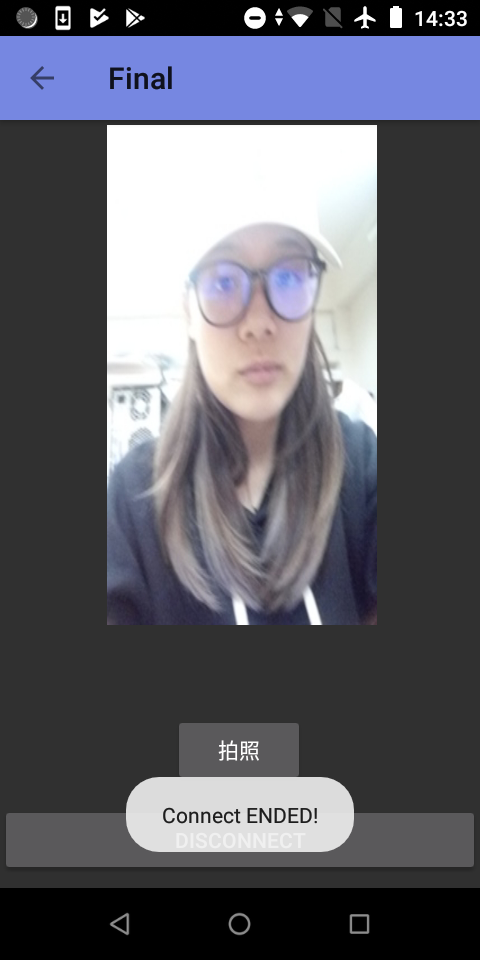
\includegraphics[scale=0.15]{pic/ch4/game05.png}
\end{itemize}

\subsection{遊戲者體驗}
遊戲者體驗之評價
\newpage

\section{結論}
在本專題中,我們所開發的遊戲優勢在於這是一個非常創新的玩法,且能在遊戲中兼具運動效果及聯絡情誼之意義。此外,本系統包含了多項技術,包括:使用快速傅立葉轉換分析肌肉感測器的訊號,利用OpenCV技術進行影像處理,透過TCP架構之網路連線即時傳送。\\
\indent 本系統所使用肌肉感測器可以貼在任何明顯肌群部位,可以更符合遊戲體驗者需求,比如從手臂更換到小腿,即可有更多不同玩法。未來,希望能增設遊戲招式之難度,且持續優化影像處理後之畫面,以及網路傳輸影像、數據之效率,提升整體遊戲品質。\\
\newpage

\section{工作分配}
\begin{tabular}{|c|c|p{9.5cm}|}
\hline
\cellcolor[HTML]{B2BEB5}姓名 & \cellcolor[HTML]{B2BEB5}內容 & \cellcolor[HTML]{B2BEB5}說明\\
\hline\hline
\multirow{5}{*}{王佳君} & 網路連線 & 建構TCP網路架構,建立伺服器端及客戶端連線 \\
\cline{2-3}
\multirow{5}{*}{} & 肌肉感測器 & 讀取Arduino數據,分析波形、判斷數據 \\
\cline{2-3}
\multirow{5}{*}{} & 系統整合 & 整合成完整系統 \\
\cline{2-3}
\multirow{5}{*}{} & 實驗測試 & 網路傳送與肌肉感測器延遲時間之評估\\
\cline{2-3}
\multirow{5}{*}{} & 報告文件 & 使用Latex撰寫專題報告及海報 \\
\hline
\multirow{4}{*}{林令婕} & 影像處理 & 利用OpenCV技術,變更影像色調及拼貼圖案等 \\
\cline{2-3}
\multirow{4}{*}{} & 系統整合 & 整合成完整系統 \\
\cline{2-3}
\multirow{4}{*}{} & 實驗測試 & 影像處理精確度及延遲之評估 \\
\cline{2-3}
\multirow{4}{*}{} & 報告文件 & 撰寫專題報告、海報內容 \\
\hline
\end{tabular}
\newpage

%\appendix
%\section{附錄}
%附錄

%\subsection{附錄1}
%附錄1

%\subsection{附錄2}
%附錄2
%\newpage

\begin{thebibliography}{99}  % The section of reference
\addcontentsline{toc}{section}{Reference}  % Add "Reference" into the table of contents
\bibitem{1}首頁介面效果\\
https://dotblogs.com.tw/starhao/2016/10/08/012050
\bibitem{2}快速傅立葉轉換\\
https://www.youtube.com/watch?v=k48iUhNkqh4 \\
https://reurl.cc/M7047K
\bibitem{3}藍芽連線\\
https://home.gamer.com.tw/creationDetail.php?sn=3671289
\bibitem{4}Session\\
https://blog.csdn.net/ZDW86/article/details/35795125
\bibitem{5}TCP連線\\
https://github.com/marselsampe/java-socket-tcp-sample
\end{thebibliography}
\newpage

\end{document} 